\subsection{Example 2.3}\label{sec:example3}

\subsubsection{Problem description}\label{subsec:example3-problem}

A Colombian agro-export firm that sells fruit-based products and coffee is planning its strategy for the next five years.
Management wants to separate the way it makes decisions about revenue from the way it makes decisions about expenses. For
the revenue side, the firm is considering two different market and pricing strategies. The first revenue strategy is a
premium positioning aimed at high-income consumers and European specialty stores, with higher prices but a stronger
dependence on favourable demand conditions. This will be called the premium revenue strategy. The second revenue strategy
is a volume-based strategy focused on larger retail chains and regional markets, with more moderate prices but more stable
volumes. This will be called the volume revenue strategy.

\medskip
For the expense side, the firm must choose how to organise its production and logistics. One option is to invest in a more
automated and contracted logistics system, which requires higher fixed costs but reduces exposure to large increases in
variable costs. This will be called the stable cost strategy. The other option is to rely on flexible outsourcing and spot
contracts for transport and inputs, which can be cheaper when global conditions are calm but much more expensive when there
are cost shocks. This will be called the flexible cost strategy. The firm must choose one revenue strategy and one cost
strategy, so it effectively chooses a combination such as premium revenue with stable costs or volume revenue with
flexible costs.

\medskip
The firm faces two independent sources of uncertainty. The first is global demand for its products, which can be high,
moderate or weak. When demand is high, if the firm chooses the premium revenue strategy it expects annual revenue of 6000,
while with the volume revenue strategy it expects annual revenue of 5500. When demand is moderate, the premium revenue
strategy is expected to generate revenue of 4500 and the volume revenue strategy revenue of 4300. When demand is weak, the
premium revenue strategy is expected to generate revenue of 3200 and the volume revenue strategy revenue of 3800. All
revenues are measured in thousands of US dollars per year. Based on market analysis, management estimates that the
probability of high demand is 0.30, the probability of moderate demand is 0.45 and the probability of weak demand is 0.25.

\medskip
The second source of uncertainty is the global cost environment, which affects production and logistics expenses. The firm
considers two possible cost conditions. In a favourable cost environment, with relatively low input and shipping costs,
yearly expenses are expected to be 2000 if the firm chooses the stable cost strategy and 1500 if it chooses the flexible
cost strategy. In an unfavourable cost environment, with high fuel prices and congested shipping routes, yearly expenses
are expected to be 2600 under the stable cost strategy and 3400 under the flexible cost strategy. These expense values are
also measured in thousands of US dollars per year. The firm estimates that the probability of favourable costs is 0.60 and
the probability of unfavourable costs is 0.40. It assumes that global demand conditions and the global cost environment are
independent.

\medskip
Annual profit is defined as revenue minus expenses. Therefore, for each year, profit is determined by the combination of
the demand scenario that occurs, the cost scenario that occurs and the pair of decisions chosen by the firm (one decision
for revenue and another for costs). Because demand and cost conditions are independent, the probability of any combined
state of nature is the product of the probability of the corresponding demand level and the probability of the
corresponding cost level. Management wants to compare the different revenue--cost combinations using several decision
rules, including Maximax, Maximin, the maximum opportunity (minimax regret) criterion and the Bayes expected value rule,
and then decide which combination of revenue strategy and cost strategy is most coherent given its preferences about risk
and its probability assessments.


\subsubsection{(C2) Interpreting the parts of the decision problem}\label{subsubsec:example3-c2}

We interpret the narrative and identify the key components of the decision situation.
\begin{table}[h!]
	\centering
	\begin{tabularx}{\linewidth}{@{}L{0.3\linewidth}Y@{}}
		\toprule
		Element & Description \\
		\midrule
		Revenue decision alternatives &
		Premium revenue strategy (higher prices, more sensitive to demand).\newline
		Volume revenue strategy (moderate prices, more stable volumes). \\
		\addlinespace
		Cost decision alternatives &
		Stable cost strategy (automation and long-term contracts, more stable expenses).\newline
		Flexible cost strategy (outsourcing and spot contracts, cheaper in calm periods but risky under cost shocks). \\
		\addlinespace
		Combined decision alternatives &
		A: Premium revenue + stable costs.\newline
		B: Premium revenue + flexible costs.\newline
		C: Volume revenue + stable costs.\newline
		D: Volume revenue + flexible costs. \\
		\addlinespace
		Independent events &
		Demand event with three levels high, moderate and weak, which determines revenue.\newline
		Cost event with two levels favourable and unfavourable, which determines expenses. \\
		\addlinespace
		States of nature &
		Each state of nature is a combination of one demand level and one cost level, for example high demand with
		favourable costs or weak demand with unfavourable costs. \\
		\addlinespace
		Probabilities &
		Demand probabilities are 0.30 for high demand, 0.45 for moderate demand and 0.25 for weak demand.\newline
		Cost probabilities are 0.60 for favourable costs and 0.40 for unfavourable costs.\newline
		Demand and cost events are independent, so each combined state’s probability is the product of the relevant demand
		probability and cost probability. \\
		\addlinespace
		Consequences &
		Annual profit in thousands of US dollars, calculated as revenue minus expenses, for each combined revenue--cost
		decision and each combined state of nature. \\
		\bottomrule
	\end{tabularx}
\end{table}

\subsubsection{(C3) Building the payoff table from the revenue and expense information}\label{subsubsec:example3-c3}

From the problem description, we first organise the revenue and expense information for each separate event and decision.
All amounts are in thousands of US dollars per year.

\medskip
\noindent Revenue as a function of demand for each revenue strategy:
\begin{table}[h!]
	\centering
	\begin{tabularx}{\linewidth}{@{}L{0.3\linewidth}C C C@{}}
		\toprule
		Demand level & Probability & Premium revenue strategy & Volume revenue strategy \\
		\midrule
		High & 0.30 & 6000 & 5500 \\
		Moderate & 0.45 & 4500 & 4300 \\
		Weak & 0.25 & 3200 & 3800 \\
		\bottomrule
	\end{tabularx}
\end{table}

\medskip
\noindent Expenses as a function of cost conditions for each cost strategy:
\begin{table}[h!]
	\centering
	\begin{tabularx}{\linewidth}{@{}L{0.3\linewidth}C C C@{}}
		\toprule
		Cost level & Probability & Stable cost strategy & Flexible cost strategy \\
		\midrule
		Favourable & 0.60 & 2000 & 1500 \\
		Unfavourable & 0.40 & 2600 & 3400 \\
		\bottomrule
	\end{tabularx}
\end{table}

Because demand and cost conditions are independent, a state of nature is described by a pair of events. We define six
combined states: S1 is high demand with favourable costs, S2 is high demand with unfavourable costs, S3 is moderate demand
with favourable costs, S4 is moderate demand with unfavourable costs, S5 is weak demand with favourable costs and S6 is
weak demand with unfavourable costs. The joint probabilities are
\[
\begin{aligned}
P(S1) &= 0.30 \cdot 0.60 = 0.18,\\
P(S2) &= 0.30 \cdot 0.40 = 0.12,\\
P(S3) &= 0.45 \cdot 0.60 = 0.27,\\
P(S4) &= 0.45 \cdot 0.40 = 0.18,\\
P(S5) &= 0.25 \cdot 0.60 = 0.15,\\
P(S6) &= 0.25 \cdot 0.40 = 0.10.
\end{aligned}
\]

Profit for each combined decision and state of nature is revenue minus expenses. We label the combined decisions as
follows: A is premium revenue with stable costs, B is premium revenue with flexible costs, C is volume revenue with stable
costs and D is volume revenue with flexible costs. For example, in S1 there is high demand and favourable costs. Under
decision A, revenue is 6000 and expenses are 2000, so profit is \(6000 - 2000 = 4000\). Under decision B, revenue is 6000
and expenses are 1500, so profit is \(6000 - 1500 = 4500\). In S6 there is weak demand and unfavourable costs. Under
decision B, revenue is 3200 and expenses are 3400, so profit is \(3200 - 3400 = -200\).

\medskip
The resulting payoff table of profit (in thousands of US dollars) is:
\begin{table}[h!]
	\centering
	\begin{tabularx}{\linewidth}{@{}L{0.12\linewidth}Y C C C C C@{}}
		\toprule
		State & Combined scenario & Probability & \shortstack{A: Premium\\stable} & \shortstack{B: Premium\\flexible} & \shortstack{C: Volume\\stable} & \shortstack{D: Volume\\flexible} \\
		\midrule
		S1 & High demand, favourable costs       & 0.18 & 4000 & 4500 & 3500 & 4000 \\
		S2 & High demand, unfavourable costs     & 0.12 & 3400 & 2600 & 2900 & 2100 \\
		S3 & Moderate demand, favourable costs   & 0.27 & 2500 & 3000 & 2300 & 2800 \\
		S4 & Moderate demand, unfavourable costs & 0.18 & 1900 & 1100 & 1700 &  900 \\
		S5 & Weak demand, favourable costs       & 0.15 & 1200 & 1700 & 1800 & 2300 \\
		S6 & Weak demand, unfavourable costs     & 0.10 &  600 & -200 & 1200 &  400 \\
		\bottomrule
	\end{tabularx}
\end{table}




\subsubsection{(C4) Maximax rule for decision making without probabilities}\label{subsubsec:example3-c4}

Under the Maximax rule, the decision maker focuses on the best possible profit of each combined decision and ignores
probabilities and worst cases.

\[
\max\{4000,\ 3400,\ 2500,\ 1900,\ 1200,\ 600\}=4000.
\]
\[
\max\{4500,\ 2600,\ 3000,\ 1100,\ 1700,\ -200\}=4500.
\]
\[
\max\{3500,\ 2900,\ 2300,\ 1700,\ 1800,\ 1200\}=3500.
\]
\[
\max\{4000,\ 2100,\ 2800,\ 900,\ 2300,\ 400\}=4000.
\]
The largest of these best profits is 4500, which corresponds to decision B in state S1. According to the Maximax rule, the
firm should choose \emph{decision B (premium revenue with flexible costs)}.

\subsubsection{(C5) Maximin rule for decision making without probabilities}\label{subsubsec:example3-c5}

Under the Maximin rule, the decision maker looks at the worst profit of each combined decision and then chooses the
decision whose worst-case outcome is the strongest.

\[
\min\{4000,\ 3400,\ 2500,\ 1900,\ 1200,\ 600\}=600.
\]
\[
\min\{4500,\ 2600,\ 3000,\ 1100,\ 1700,\ -200\}=-200.
\]
\[
\min\{3500,\ 2900,\ 2300,\ 1700,\ 1800,\ 1200\}=1200.
\]
\[
\min\{4000,\ 2100,\ 2800,\ 900,\ 2300,\ 400\}=400.
\]
We compare these worst-case values and choose the highest one,
\[
\max\{600,\ -200,\ 1200,\ 400\}=1200.
\]
Under the Maximin rule, the firm should choose \emph{decision C (volume revenue with stable costs)}, because it offers the
strongest worst-case profit.

\subsubsection{(C6) Maximum opportunity criterion (minimax regret)}\label{subsubsec:example3-c6}

The maximum opportunity or minimax regret criterion focuses on regret, defined as the loss from not having chosen the best
decision in a given state of nature. For each state, we identify the best profit and then compute regret as the best profit
in that state minus the profit of the chosen decision.

\[
\begin{aligned}
\text{S1}&\colon \max\{4000,\ 4500,\ 3500,\ 4000\}=4500,\\
\text{S2}&\colon \max\{3400,\ 2600,\ 2900,\ 2100\}=3400,\\
\text{S3}&\colon \max\{2500,\ 3000,\ 2300,\ 2800\}=3000,\\
\text{S4}&\colon \max\{1900,\ 1100,\ 1700,\ 900\}=1900,\\
\text{S5}&\colon \max\{1200,\ 1700,\ 1800,\ 2300\}=2300,\\
\text{S6}&\colon \max\{600,\ -200,\ 1200,\ 400\}=1200.
\end{aligned}
\]

The regret table in thousands of US dollars is:
\begin{table}[h!]
	\centering
	\begin{tabularx}{\linewidth}{@{}L{0.12\linewidth}Y C C C C@{}}
		\toprule
		State & Scenario & A Regret & B Regret & C Regret & D Regret \\
		\midrule
		S1 & High demand, favourable costs & \(4500-4000=500\) & \(4500-4500=0\) & \(4500-3500=1000\) & \(4500-4000=500\) \\
		S2 & High demand, unfavourable costs & \(3400-3400=0\) & \(3400-2600=800\) & \(3400-2900=500\) & \(3400-2100=1300\) \\
		S3 & Moderate demand, favourable costs & \(3000-2500=500\) & \(3000-3000=0\) & \(3000-2300=700\) & \(3000-2800=200\) \\
		S4 & Moderate demand, unfavourable costs & \(1900-1900=0\) & \(1900-1100=800\) & \(1900-1700=200\) & \(1900-900=1000\) \\
		S5 & Weak demand, favourable costs & \(2300-1200=1100\) & \(2300-1700=600\) & \(2300-1800=500\) & \(2300-2300=0\) \\
		S6 & Weak demand, unfavourable costs & \(1200-600=600\) & \(1200-(-200)=1400\) & \(1200-1200=0\) & \(1200-400=800\) \\
		\bottomrule
	\end{tabularx}
\end{table}

For each decision, we identify its maximum regret across all states:
\[
\begin{aligned}
\max \text{Regret}(A) &= \max\{500,\ 0,\ 500,\ 0,\ 1100,\ 600\}=1100,\\
\max \text{Regret}(B) &= \max\{0,\ 800,\ 0,\ 800,\ 600,\ 1400\}=1400,\\
\max \text{Regret}(C) &= \max\{1000,\ 500,\ 700,\ 200,\ 500,\ 0\}=1000,\\
\max \text{Regret}(D) &= \max\{500,\ 1300,\ 200,\ 1000,\ 0,\ 800\}=1300.
\end{aligned}
\]
The minimax regret rule chooses the decision with the smallest of these maximum regrets, which is decision C. The maximum
opportunity criterion therefore recommends \emph{decision C (volume revenue with stable costs)}.

\subsubsection{(C7) Using probabilities and expected value (Bayes decision rule)}\label{subsubsec:example3-c7}

The Bayes decision rule with expected monetary value (EMV) multiplies each profit by the probability of its state and adds
the results. We use the joint probabilities of S1 to S6.

\[
\begin{aligned}
EMV_A &= 0.18(4000) + 0.12(3400) + 0.27(2500) + 0.18(1900) + 0.15(1200) + 0.10(600) \\
&= 720 + 408 + 675 + 342 + 180 + 60 = 2385.
\end{aligned}
\]
\[
\begin{aligned}
EMV_B &= 0.18(4500) + 0.12(2600) + 0.27(3000) + 0.18(1100) + 0.15(1700) + 0.10(-200) \\
&= 810 + 312 + 810 + 198 + 255 - 20 = 2365.
\end{aligned}
\]
\[
\begin{aligned}
EMV_C &= 0.18(3500) + 0.12(2900) + 0.27(2300) + 0.18(1700) + 0.15(1800) + 0.10(1200) \\
&= 630 + 348 + 621 + 306 + 270 + 120 = 2295.
\end{aligned}
\]
\[
\begin{aligned}
EMV_D &= 0.18(4000) + 0.12(2100) + 0.27(2800) + 0.18(900) + 0.15(2300) + 0.10(400) \\
&= 720 + 252 + 756 + 162 + 345 + 40 = 2275.
\end{aligned}
\]
These values are expected annual profits in thousands of US dollars. Since \(EMV_A = 2385\) is the highest expected value,
the Bayes EMV rule recommends \emph{decision A (premium revenue with stable costs)}.

\subsubsection{(C9) Tree diagram of the decision-making problem}\label{subsubsec:example3-c9}

The same decision situation can be represented as a decision tree. The firm first chooses a combined decision (revenue
strategy and cost strategy), then the demand level is realised and then the cost level is realised. Because demand and
costs are independent, their probabilities multiply along each path. For simplicity, we show the combined states with their
joint probabilities and profits.
\begin{center}
	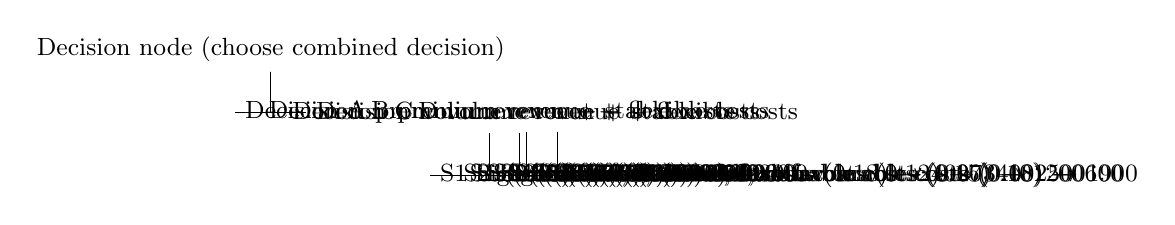
\begin{tikzpicture}[
		grow=down,
		level distance=8mm,
		sibling distance=3mm,
		edge from parent/.style={draw},
		edge from parent path={(\tikzparentnode.south) |- (\tikzchildnode.west)},
		every node/.style={anchor=west,font=\small}
	]
		\node {Decision node (choose combined decision)}
			child { node {Decision A premium revenue + stable costs}
				child { node {S1 high demand, favourable costs (0.18) $\to$ 4000} }
				child { node {S2 high demand, unfavourable costs (0.12) $\to$ 3400} }
				child { node {S3 moderate demand, favourable costs (0.27) $\to$ 2500} }
				child { node {S4 moderate demand, unfavourable costs (0.18) $\to$ 1900} }
				child { node {S5 weak demand, favourable costs (0.15) $\to$ 1200} }
				child { node {S6 weak demand, unfavourable costs (0.10) $\to$ 600} }
			}
			child { node {Decision B premium revenue + flexible costs}
				child { node {S1 (0.18) $\to$ 4500} }
				child { node {S2 (0.12) $\to$ 2600} }
				child { node {S3 (0.27) $\to$ 3000} }
				child { node {S4 (0.18) $\to$ 1100} }
				child { node {S5 (0.15) $\to$ 1700} }
				child { node {S6 (0.10) $\to$ -200} }
			}
			child { node {Decision C volume revenue + stable costs}
				child { node {S1 (0.18) $\to$ 3500} }
				child { node {S2 (0.12) $\to$ 2900} }
				child { node {S3 (0.27) $\to$ 2300} }
				child { node {S4 (0.18) $\to$ 1700} }
				child { node {S5 (0.15) $\to$ 1800} }
				child { node {S6 (0.10) $\to$ 1200} }
			}
			child { node {Decision D volume revenue + flexible costs}
				child { node {S1 (0.18) $\to$ 4000} }
				child { node {S2 (0.12) $\to$ 2100} }
				child { node {S3 (0.27) $\to$ 2800} }
				child { node {S4 (0.18) $\to$ 900} }
				child { node {S5 (0.15) $\to$ 2300} }
				child { node {S6 (0.10) $\to$ 400} }
			};
	\end{tikzpicture}
\end{center}


This diagram makes explicit the sequence of decisions and uncertain events, as well as the joint probabilities and
profits associated with each possible path.

\subsubsection{(C8) Comparing Bayes, Maximin, Maximax and minimax regret}\label{subsubsec:example3-c8}

We summarise the recommendations from the different decision rules:
\begin{itemize}
	\item Maximax, which is very optimistic and focuses on the best possible profit, recommends decision B (premium revenue + flexible costs) because it can reach 4500.
	\item Maximin, which is very cautious and focuses on the worst-case profit, recommends decision C (volume revenue + stable costs) because its worst case is 1200.
	\item The maximum opportunity or minimax regret rule, which focuses on limiting the largest possible regret, recommends decision C because its maximum regret is 1000, smaller than the maximum regrets of A, B and D.
	\item The Bayes EMV rule, which uses the full joint distribution of probabilities and profits, recommends decision A (premium revenue + stable costs) because it has the highest expected monetary value, 2385.
\end{itemize}
The comparison shows that rules ignoring probabilities and focusing on extreme outcomes can produce different
recommendations from rules that use all probability information. Decision B is favoured by a very optimistic view,
decision C by a very cautious view and by regret minimisation, while decision A is favoured by the expected value
criterion.

\subsubsection{(C10) Evaluating all possibilities in the decision problem}\label{subsubsec:example3-c10}

Looking across all rules, the firm can evaluate each combined decision in terms of risk and reward. Decision A, premium
revenue with stable costs, offers strong profits in favourable states without negative outcomes and achieves the highest
expected profit, but it does not have the strongest worst-case profit. Decision B, premium revenue with flexible costs, has
the highest possible profit when demand is high and costs are favourable but exposes the firm to a negative profit of -200
when demand is weak and costs are unfavourable, and therefore has a high maximum regret. Decision C, volume revenue with
stable costs, never performs extremely badly or extremely well. It offers the strongest worst-case profit and the smallest
maximum regret, but its expected value is somewhat lower than that of decision A. Decision D, volume revenue with flexible
costs, lies between the others in many states but does not dominate any of them in terms of either expected value, worst
case or regret. This evaluation highlights how attitudes towards risk, regret and the role of probabilities lead to
different recommended actions, and how separating revenue and expense decisions creates a richer set of trade-offs.

\subsubsection{(C1) Formulating the final decision and summarising all criteria}\label{subsubsec:example3-c1}

Based on each of the decision criteria used in the solution, the recommended combined decision would be as follows. If the
firm decides according to the Maximax rule and adopts a highly optimistic and risk-seeking attitude, it should choose
decision B, premium revenue with flexible costs, because this combination can reach the highest profit among all combined
states. If the firm decides according to the Maximin rule and wants to protect itself against the worst possible profit, it
should choose decision C, volume revenue with stable costs, because this combination has the strongest worst-case outcome.
If the firm uses the maximum opportunity or minimax regret criterion and cares mainly about limiting the largest possible
regret from a wrong choice, it should again choose decision C, since its maximum regret is the smallest among all options.
If the firm trusts the estimated probabilities for demand and cost conditions and uses the Bayes expected value rule to
maximise expected annual profit, it should choose decision A, premium revenue with stable costs, because this combination
has the highest expected monetary value.

\medskip
The decision tree representation confirms how the two independent events, demand and costs, interact with the two separate
decisions on revenue and expenses. The comparison and evaluation clarify how each decision rule reflects a particular
attitude toward risk and uncertainty. Taking all criteria together, a coherent summary conclusion is that decision A,
premium revenue with stable costs, is the most attractive option for a firm that wants to maximise expected profit while
avoiding extreme downside risk, whereas decision C, volume revenue with stable costs, is more appropriate for a firm that
prioritises robustness of the worst-case outcome and regret minimisation. For a firm that wishes to use probability
information responsibly but still give weight to security, stating its final decision as choosing premium revenue with
stable costs and clearly understanding how this differs from the more conservative choice volume revenue with stable costs
is consistent with the overall analysis of this two-decision problem.

\medskip
\noindent\hyperref[sec:example3]{Back to top}
